\chapter{Exploratory Data Analysis}

\section{Data Formats}

\noindent The reports can be requested from the CDP website \cite{CDPMain2024}, they available both in PDF and a structured CSV format. The CSV files encompass the responses submitted to the CDP questionnaire, which form the foundation of the predictor and response variables for this thesis. My work is a continuation of the initial data processing that was executed by Climate and Sustainability Impact Lab \cite{HarvardD3Lab2024} and kindly shared with me in the form of various stata files and a repository containg both the raw and processed data, where the multiple sections had been extracted from the survey and aligned across different years. I then imported all the data and further processed it to create the training and tests sets for the following models. 

\section{CDP Report Structure}
The CDP survey has $X$ primary sections, with each section containign a list of subsecitons with relevant questions. This is a list of the primary sections as well as a brief introduction to the types of questions present in the section:
\begin{itemize}
    \item \textbf{C0 - Introduction:} General description of the organization, along with information on where the company operates geographically, the currency used to report financial information, and the reporting boundary (whether it is financial or operational control), and the ISIN if the company is public
    \item \textbf{C1 - Governance:} Governance structures and processes related to climate change within the organization. It includes questions about board-level oversight of climate-related issues, the roles and responsibilities of management in addressing climate change, and how climate-related risks and opportunities are integrated into the company's overall governance framework. This section provides insight into the company's commitment to addressing climate change at the highest level of its organizational structure.
    \item \textbf{C2 - Risks and Opportunities:} Identification of processes that the organization uses to identify, assess, and respond to climate-related risks and opportunities. It includes questions regarding the definition of time horizons (short, medium, and long-term) for these risks and opportunities, and specific related details. This section aims to understand how the company perceives and manages potential impacts of climate change on its business, highlighting its approach to mitigating risks and capitalizing on new opportunities arising from the changing climate landscape.
    \item \textbf{C3 - Business Strategy:} This section examines the company's business strategy in relation to climate change. It explores whether the organization's strategy includes a transition plan that aligns with a 1.5°C world scenario, detailing the nature and publicly available aspects of this plan. The focus is on understanding how the company's strategy is designed to adapt to and mitigate climate-related issues, and how it plans to transition towards a lower-carbon, more sustainable business model. This section also looks at how feedback is collected from shareholders on the transition plan, emphasizing the integration of climate considerations into the core business strategy.
    \item \textbf{C4 - Targets and Performance:} This section presents an in-depth analysis of the company's specific emissions targets, including which emissions scopes are covered, targeted reduction percentages, and the current progress towards these goals. It also examines the emissions reduction initiatives that the company had active during the reporting year, detailing associated investments and the expected payback period. This part of the report effectively illustrates both the targets set by the company for reducing emissions and the concrete initiatives underway to achieve these objectives.
    \item \textbf{C5 - Emissions Methodology:} Insights into the company's emissions methodology, including any structural changes that may have occurred. It outlines the base year emissions against which progress is measured and explains the methodology employed to collect and report emission data. Additionally, it highlights the protocols and standards adhered to, ensuring the accuracy, consistency, and comparability of emissions data over time.
    \item \textbf{C6 - Emissions Data}: This section covers both Scope 1 and Scope 2 emissions. It includes relevant details, such as the categorization of Scope 2 emissions as either location-based or market-based. Additionally, the section provides insights into emission intensity per product, allowing for a detailed examination of emissions in relation to the company's products and operations. 
    \item \textbf{C7 - Emissions Breakdowns:} This is the section where company emissions (scope 1 and 2) are broken down into various sub-categories based on country/region, business division, and sector production activity. Most importantly, this section also provides a \underline{breakdown of changes in gross global emissions} (Scope 1 and 2 combined), and for each of them a specification of how your emissions compare to the previous year. \textbf{Emissions breakdowns will be further analyzed in the response variable discussion and linked to this section.}
    \item \textbf{C8 - Energy:} A comprehensive description of energy purchases and consumption, with a specification of renewable and non-renewable sources as well as consumption breakdowns by location. This section is useful in understanding whether the company is actively purchasing renewable energy and whether the firm's activity are energy intensive. 
    \item \textbf{C9 - Additional metrics:} Description of other sustainability related metrics such as investments in low carbon research and developement, transport technologies, and product/services
    \item \textbf{C10 - Verification:} This section provides a comprehensive description of the verification methodologies that the firm implements to verify and audit its emissions scopes. The report includes the proportion of verified emissions by scopes, verification standards and status.
    \item \textbf{C11 - Carbon Pricing:} Assesment of whether the company is subjected to a carbon tax and, if so, in which geographies and under which regimes along with a description of the percentage of emission scopes covered by the policy and the strategies that the company is implementing to comply with the regulations. Additionally, the section asks whether the company has an internal price of carbon and its related objectives.
    \item \textbf{C12 - Engagement:} Analysis of the company's effort to engage with its value chain to reduce carbon emissions. In particular, the company discloses which agents does the company collaborate with, whether the company requires suppliers to meet certain sustainability criteria, and whether the company engages with customers to drive awareness on climate related issues. Additionally, the company discloses whether it engages with policy makers in a way that could influence climate related policy, law, or regulation
    \item \textbf{Other Sections:} Sections beyond C$12$ are not relevant for the purpose of the thesis. They include details on biodiversity and signoff details among other metrics.
\end{itemize}

\section{A Case Study on Two CDP Reports}

\noindent To begin the discussion on exploratory data analysis, I must first address the complexities of emission accounting and reporting within the framework of CDP data, highlighting its distinct nature compared to the more standardized field of financial reporting. That is, despite ongoing improvements, emission reporting still falls short of the robust standards established in financial accounting. I will highlight this by analyzing the 2022 CDP reports from two markedly different companies: General Motors (GM) in the automotive sector and Jet Blue in the airline industry. These reports underscore the highly company-specific nature of emission data, with significant variances stemming from diverse operational practices, especially across different industries. This results in a substantial reliance on text-based and free-form answers within the CDP reports, presenting unique challenges for data analysis. To navigate this complexity, a critical starting point is to analyze the inherent differences in these reports, which will inform and refine our modeling approach. By understanding and accommodating these industry-specific nuances, we aim to develop a more accurate and representative model of emission reporting and reduction strategies as well as identifying potential areas of improvement. 

\subsection{General Motors 2022 CDP Report}
General Motors Company (GM), a global leader in the automotive industry, is headquartered in Detroit, Michigan, USA. Renowned for its ownership and production of the Chevrolet, GMC, Cadillac, and Buick brands, GM was the largest automaker in the United States by sales in 2022. GM's commitment to sustainability is evident in its strategic approach to reducing Scope 1, Scope 2, and Scope 3 greenhouse gas (GHG) emissions, with comprehensive governance and ambitious environmental targets.

\subsection*{Scope 1 and Scope 2 Emissions}
GM has set forth aggressive targets to reduce its Scope 1 and Scope 2 emissions by 71.4\% by 2035, relative to its 2018 baseline. In 2018, GM reported Scope 1 emissions of 1,763,555 metric tons CO2e and Scope 2 emissions of 3,924,338 metric tons CO2e. By the reporting year 2022, GM achieved a reduction to 1,252,906 metric tons CO2e for Scope 1 and 2,150,694 metric tons CO2e for Scope 2, marking significant progress towards its goal. This reduction aligns with the 1.5 degrees Celsius strategy set by the Paris Agreement, underscoring GM's commitment to global climate initiatives \cite{GeneralMotorsWikipedia, Zhou2020Decarbonization}.

GM's strategy includes enhancing energy efficiency across its manufacturing operations and increasing the use of renewable energy. In 2021, GM implemented over 300 energy efficiency improvements, such as upgrading to more efficient equipment and increasing renewable electricity use from 23\% to 25\%, contributing to GHG reductions in Scope 2 emissions.

\subsection*{Scope 3 Emissions}
Addressing Scope 3 emissions, GM has set a target to achieve a 50.4\% reduction in its vehicle use emissions, from a baseline of 0.0002466 metric tons of CO2 per kilometer to 0.0001223136. GM's strategy to meet this target includes transitioning to an all-electric vehicle (EV) future, with plans to introduce 30 new EV models by 2025 and aspirations to be fully electric by 2035. Partnerships to increase renewable energy generation and deploy EV chargers, in collaboration with EvGo, further exemplify GM's holistic approach to reducing its carbon footprint across the value chain.

\subsection*{Key Takeaways}
\begin{itemize}
    \item \textbf{Strategic Emissions Reduction:} GM's targeted reductions in Scope 1 and Scope 2 emissions demonstrate a strong commitment to environmental stewardship, leveraging technological advancements and renewable energy.
    \item \textbf{Leadership in Electric Vehicles:} GM's aggressive transition to an all-EV lineup by 2035 highlights its leadership role in transforming the automotive industry towards sustainability.
    \item \textbf{Comprehensive Approach to Sustainability:} Through its Scope 3 emissions reduction target, GM addresses the broader environmental impact of its products, emphasizing the importance of a comprehensive strategy that extends beyond direct emissions.
\end{itemize}

GM's sustainability efforts showcase a deep commitment to reducing its environmental impact and leading the automotive industry towards a more sustainable future. By strategically targeting Scope 1, Scope 2, and Scope 3 emissions, GM is not only adhering to global climate agreements but also setting a precedent for corporate responsibility in addressing climate change.


% \subsection{General Motors' Report Analysis}

% \noindent General Motors Company (GM), an American multinational automotive manufacturing giant, is headquartered in Detroit, Michigan, USA. Esteemed for its ownership and production of four prominent automobile brands—Chevrolet, GMC, Cadillac, and Buick—it stood as the largest automaker in the United States by sales in 2022 \cite{GeneralMotorsWikipedia}. At the core of GM's corporate strategy lies a robust sustainability framework, spearheaded at the enterprise level. This framework encompasses oversight by the Board, the Chief Executive Officer, and the Chief Sustainability Officer, alongside a dedicated Board-level committee tasked with addressing climate-related challenges. Furthermore, the company has instituted a monetary incentive for its corporate executive team, primarily tethered to the deployment and success of its electric vehicle (EV) fleet.

% \noindent In pursuit of environmental sustainability, GM has set ambitious targets to reduce its Scope 1 and Scope 2 emissions by 71.4\% by 2035, relative to its 2018 baseline, where emissions were recorded at 1,763,555 and 3,924,338 metric tons CO2e for Scope 1 and Scope 2, respectively. As of 2022, the company has realized 56.24\% of this target, with reported emissions of 1,252,906 for Scope 1 and 2,150,694 for Scope 2, aligning with the 1.5 degrees Celsius strategy of the Paris Agreement \cite{Zhou2020Decarbonization}. GM's progress is attributed to enhanced energy efficiency in its manufacturing processes and a strategic shift towards renewable energy procurement.

% \noindent The company's sustainability report highlights the implementation of over 300 energy efficiency improvements in 2021 across its buildings and processes. These include the adoption of more efficient equipment, such as variable speed drives on motors, process controls, LED lighting, among other conservation measures. Additionally, GM increased its renewable electricity usage from 23\% to 25\%, further contributing to reductions in Scope 2 market-based emissions. This approach exemplifies how the automotive industry can effectively reduce emissions through renewable energy adoption and manufacturing efficiencies, a stark contrast to sectors like cement production, which accounts for 7\% of global anthropogenic greenhouse gas emissions and faces significant decarbonization challenges due to the inherent CO2 generation during limestone calcination \cite{Ostovari2021}.

% \noindent However, the most daunting challenge for GM lies within Scope 3 emissions, predominantly stemming from vehicle use and fossil fuel combustion. While the company has not provided an estimate for its Scope 3 emissions, it aims to reduce these emissions by 50.4\% from a baseline of 0.0002466 metric tons of CO2 per kilometer to 0.0001223136. Achieving this reduction is contingent upon GM's strategic pivot to an all-EV future, underscored by its commitment to launch 30 new EV models by 2025, transition entirely to EVs by 2035, and bolster renewable energy generation and EV charger deployment in collaboration with EvGo, a leading charging network, with an aim to power these chargers entirely by renewable energy. This strategy underscores the critical insights for the automotive industry:
% \begin{itemize}
%     \item Scope 3 emissions, primarily from vehicle use, constitute the most significant share of emissions, presenting the greatest reduction challenge.
%     \item GM is actively enhancing its production processes and renewable energy initiatives, demonstrating tangible success in emission reduction efforts.
%     \item The reduction of Scope 3 emissions hinges on a more complex strategy, currently in its nascent stages, with GM having achieved only 0.225\% progress toward its target, underscoring the enormity of the challenge ahead.
% \end{itemize}

\subsection{JetBlue Airways Corporation 2022 CDP Report}
JetBlue Airways Corporation has been steadfast in its commitment to environmental stewardship, focusing on reducing Scope 1, Scope 2, and Scope 3 greenhouse gas (GHG) emissions across its operations. The airline's governance structure emphasizes sustainability, with strategic initiatives overseen by its board and executive team, underscoring a comprehensive approach to addressing climate change.

\subsection*{Scope 1 and Scope 2 Emissions}
In the reporting year 2022, JetBlue's Scope 1 emissions totaled 6,853,927 metric tons CO2e, predominantly from jet fuel combustion, a primary challenge within the airline industry. Scope 2 emissions amounted to 25,945 metric tons CO2e, reflecting the emissions from electricity consumption. These figures demonstrate JetBlue's significant environmental footprint, necessitating aggressive measures for reduction.

\noindent JetBlue's strategies to mitigate these emissions include modernizing its fleet with more fuel-efficient aircraft, such as the Airbus A220 and A321neo, and investing in sustainable aviation fuel (SAF) to reduce lifecycle GHG emissions associated with jet fuel. Additionally, the airline is transitioning its ground service equipment to electric power, aligning with its commitment to lower Scope 1 and Scope 2 emissions.

\subsection*{Scope 3 Emissions}
JetBlue's Scope 3 emissions are a crucial component of its sustainability strategy, addressing emissions from purchased goods and services, capital goods, and fuel-and-energy-related activities not included in Scope 1 or 2. In 2022, the emissions reported were as follows:

\begin{itemize}
    \item Purchased Goods and Services: 44,922 metric tons CO2e, estimated for catered food and onboard product.
    \item Capital Goods: 485,629 metric tons CO2e, associated with aircraft ground equipment and spare parts.
    \item Fuel-and-Energy-Related Activities: 1,391,126 metric tons CO2e, highlighting the broader impact of JetBlue's operational energy use.
\end{itemize}

\noindent These figures were calculated using the Quantis Scope 3 tool, demonstrating JetBlue's reliance on standardized methodologies to quantify and manage its indirect emissions. The airline's commitment to understanding and reducing its Scope 3 emissions is evident through its detailed reporting and targeted reduction strategies, including investments in SAF and efficiency improvements across its value chain.

\subsection*{Key Takeaways}
\begin{itemize}
    \item \textbf{Comprehensive Climate Strategy:} JetBlue's efforts to reduce Scope 1, Scope 2, and Scope 3 emissions underscore a holistic approach to sustainability, addressing both direct and indirect sources of GHG emissions.
    \item \textbf{Innovation and Efficiency:} Through fleet modernization, SAF investments, and operational efficiencies, JetBlue is actively working towards reducing its environmental impact, despite the inherent challenges of the airline industry.
    \item \textbf{Scope 3 Emissions Challenge:} JetBlue's detailed reporting on Scope 3 emissions highlights the complexity of addressing indirect emissions. The airline's engagement with its supply chain and investment in sustainable practices exemplify a forward-thinking approach to environmental responsibility.
\end{itemize}

\noindent JetBlue's sustainability efforts reflect a deep commitment to reducing its carbon footprint and contributing to the global fight against climate change. By addressing Scope 1, Scope 2, and Scope 3 emissions with targeted strategies and investments, JetBlue is paving the way for a more sustainable future in aviation.


\newpage
\section{Data Description}

\begin{forest}
    for tree={
        draw,
        rounded corners,
        align=center,
        edge={->},
        parent anchor=south,
        child anchor=north,
        s sep+=1.6cm, % Increased vertical spacing
        l sep+=1.1cm, % Increase the level distance
    },
    [CDP Climate Response Survey Data\\\textbf{34,588 firm-years}, fill=blue!20
        [Frim has an ISIN code?, edge, fill=yellow!20
            [\textbf{24,803 firm-years}, edge label={node[midway, above left] {YES}}, fill=green!20
                [Is Worldscope and GICS data available?, edge, fill=yellow!20
                    [\textbf{19,200 firm-years}, edge label={node[midway, above left] {YES}}, fill=green!20
                        [Is CDP control data available?, edge, fill=yellow!20
                            [\underline{\textbf{18,491 firm-years}}, edge label={node[midway, above right] {YES}}, fill=green!20]
                            [\text{709} firm-years dropped, edge label={node[midway, above right] {NO}}, fill=red!20]
                        ]
                    ]
                    [\text{5,603} firm-years dropped, edge label={node[midway, above right] {NO}}, fill=red!20]
                ]
            ]
            [\text{9,785} firm-years dropped, edge label={node[midway, above right] {NO}}, fill=red!20]
        ]
    ]
\end{forest}










\begin{itemize}
    \item Number of firms and unique isins
    \item Number of variables
    \item Number of firms per sector
\end{itemize}

\section{Response Variable Analysis}

\section{Predictor Variable Analysis}
\begin{itemize}
    \item Here I can put cool visualizations
    \item Here I can start explainig the data
    \item Here I can take inspiration from Kaggle
    \item Here is can do some clustering?
\end{itemize}
\section{Building the training set}

    
Lorem ipsum dolor sit amet, consectetuer adipiscing elit. Morbi commodo, ipsum sed pharetra gravida, orci magna rhoncus neque, id pulvinar odio lorem non turpis. Nullam sit amet enim. Suspendisse id velit vitae ligula volutpat condimentum. Aliquam erat volutpat. Sed quis velit. Nulla facilisi. Nulla libero. Vivamus pharetra posuere sapien. 

Some nice graphs are shown in Figure~\ref{fig:label2}.

\begin{figure}[htbp]
\begin{center}
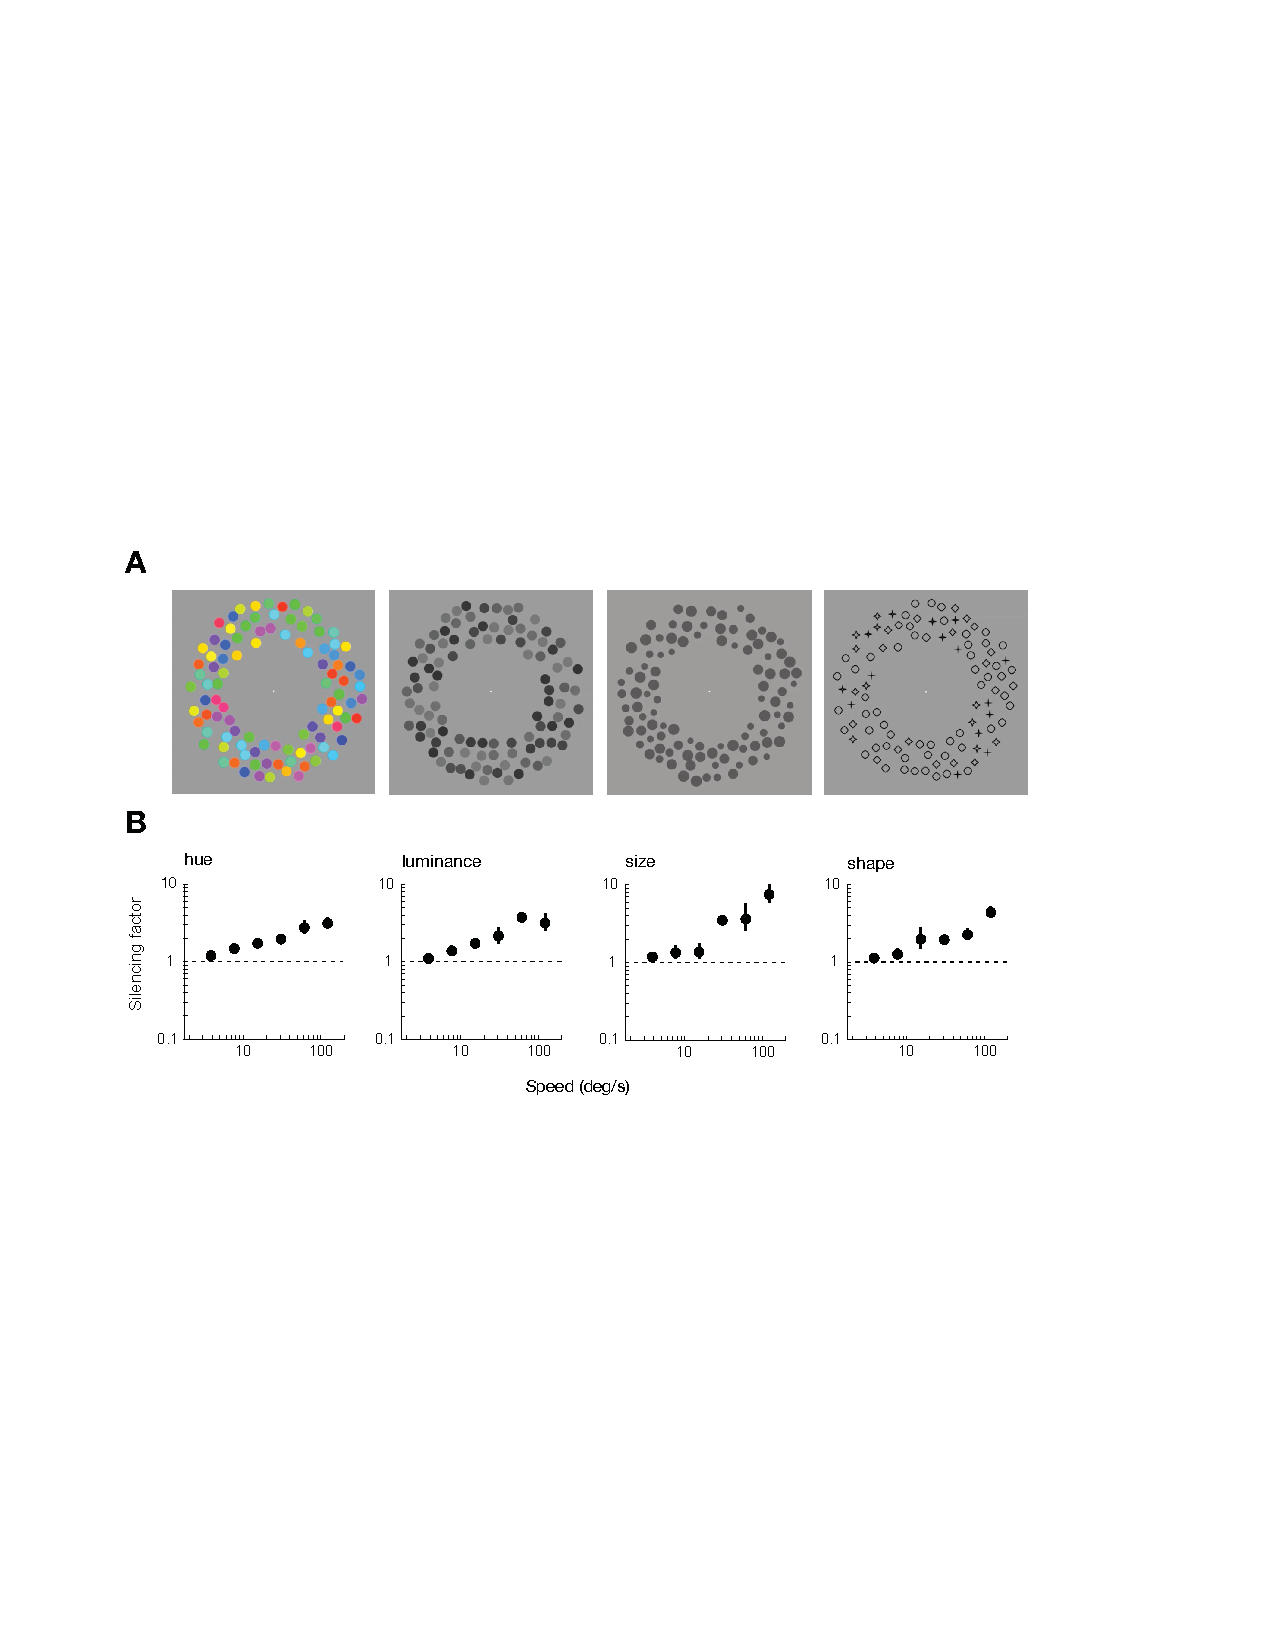
\includegraphics[width=4in]{figures/fig1.pdf}
\caption{Some nice graphs.}
\label{fig:label2}
\end{center}
\end{figure}